\RequirePackage{etex}
\RequirePackage{easymat}




\documentclass[usenames,dvipsnames]{beamer}

\usepackage{amsthm,ulsy,amsmath,amssymb,
MnSymbol,tikz,bbold}
\usepackage[all]{xy}
\usepackage[active]{srcltx}
\sloppy
 \usetheme{berlin}
\setbeamertemplate{navigation symbols}{}


\renewcommand{\le}{\leqslant}
\renewcommand{\ge}{\geqslant}

\renewcommand{\dashrightarrow}
{\text{\raisebox{0.9mm} {\
\begin{tikzpicture}[->,thick,xscale=0.56]
  \draw[dashed] (0,0)--(1,0)
;
\end{tikzpicture}}\ }}

\renewcommand{\dashleftarrow}
{\text{\raisebox{0.9mm} {\
\begin{tikzpicture}[<-,thick,xscale=0.56]
  \draw[dashed] (0,0)--(1,0)
;
\end{tikzpicture}}\ }}


\setcounter{page}{2}
\usepackage{color}

\definecolor{lavand}{RGB}{51,0,102}
\mode<presentation>

\begin{document}




\begin{frame}

\frametitle{
\includegraphics<1>[height=1.2cm]{configuracion_1.png}
\hspace{5cm}
\includegraphics<1>[height=1.2cm]{upc.png}
\hspace{0.3cm}
\includegraphics<1>[height=1.2cm]{knu.jpg}
}
\begin{center}
\bigskip

{\Large\alert{
Generalizations of Roth's criteria
for solvability \\
of matrix equations}}
\bigskip

{\large
{\it Tetiana Klymchuk}}\\
\medskip

{\large
{Universitat Polit\`{e}cnica de Catalunya}}\\
\vspace{1cm}


\textcolor{lavand}{\large
XXV CEDYA / XV CMA}\\
\medskip

\textcolor{lavand}{June 26--30, 2017}

\end{center}

\end{frame}







\begin{frame}
\frametitle{Semilinear mappings}

A mapping ${\cal A}$ from a complex
vector space $U$ to a complex vector
space $V$ is \alert{semilinear} if
\[
{\cal A}(u+u')={\cal A}u+{\cal A}u',\qquad
{\cal A}(\alpha u)=\alert{\bar\alpha} {\cal A}u
\]
for all $u,u'\in U$ and $\alpha
\in\mathbb C$.
\bigskip



We write
\begin{itemize}
  \item ${\cal A}:
      U\alert{\longrightarrow} V$
      if ${\cal A}$ is a
      \textcolor{blue}{linear
mapping}, and
  \item ${\cal A}:
      U\alert{\dashrightarrow} V$
      if ${\cal A}$ is a
      \textcolor{blue}{semilinear
      mapping}.
\end{itemize}
\end{frame}



\begin{frame}
\frametitle{Cycles of linear and
semilinear mappings}


We give a canonical form of matrices of
a \alert{cycle of linear and semilinear
mappings}
\[
\xymatrix{
{V_1}
\ar@{-}@/_1.5pc/[rrrr]^{\mathcal A_t}
\ar@{-}[r]^{\mathcal A_1}&
V_2\ar@{-}[r]^{\mathcal A_2\ } &
{\ \dots\ }&{V_{t-1}}
\ar@{-}[l]_{\mathcal A_{t-2}}
\ar@{-}[r]^{\ \mathcal A_{t-1}}&{V_t}}
\]
in which \textcolor{blue}{each line is}
\begin{itemize}
  \item a full arrow
      \alert{$\longrightarrow$},
      \alert{$\longleftarrow$}, or
  \item a dashed arrow
      \alert{$\dashrightarrow$},
      \alert{$\dashleftarrow$}.
\end{itemize}


\end{frame}



\begin{frame}
\frametitle{My talk is based on:}

\begin{itemize}

  \item \alert{T. Klimchuk,
  D. Kovalenko, T. Rybalkina,
  V.V. Sergeichuk}, {\it Tame systems
  of linear and semilinear mappings}),
   Contemp. Math. 658 (2016) 103-114.
\bigskip
\bigskip


  \item \alert{D. Duarte de
      Oliveira, V. Futorny, T.
      Klimchuk, D. Kovalenko, V.V.
      Sergeichuk}, {\it Cycles of
      linear and semilinear
      mappings}), Linear Algebra
      Appl. 438 (2013) 3442-3453.
\bigskip
\bigskip

  \item \alert{D. Duarte de
      Oliveira, R.A. Horn, T.
      Klimchuk, V.V. Sergeichuk},
      {\it Remarks on the
      classification of a pair of
      commuting semilinear
      operators}, Linear Algebra
      Appl. 436 (2012) 3362-3372.



\end{itemize}



\end{frame}

\begin{frame}
\frametitle{Empty matrices}

\begin{itemize}
  \item $\forall n=0,1,2,\dots$
      $\exists !$ matrices of sizes
      \alert{$0\times n$} and
      \alert{$n\times 0$},

      which correspond to linear
  mappings
  \textcolor{blue}{$\mathbb C^n\to
  0$} and
  \textcolor{blue}{$0\to\mathbb
      C^n$}.
\medskip

  \item They are denoted by
      \alert{$0_{0n}$} and
      \alert{$0_{n0}$} and are
      considered as zero matrices
\medskip

  \item For every $p\times q$
      matrix $M_{pq}$:
\begin{align*}
\alert{M_{pq}\oplus 0_{n0}}&=\begin{bmatrix}
  M_{pq} & 0 \\
  0 &0_{n0}
\end{bmatrix}=\begin{bmatrix}
  M_{pq}& 0_{p0} \\
  0_{nq}& 0_{n0}
\end{bmatrix}=\alert{\begin{bmatrix}
M_{pq} \\ 0_{nq}
\end{bmatrix}}
\\[5mm]
\alert{M_{pq}\oplus 0_{0n}}&=\begin{bmatrix}
  M_{pq} & 0 \\
  0 & 0_{0n}
\end{bmatrix}=\begin{bmatrix}
  M_{pq}& 0_{pn} \\
  0_{0q}& 0_{0n}
\end{bmatrix}=\alert{\begin{bmatrix}
   M_{pq} & 0_{pn}
\end{bmatrix}}
\end{align*}

\end{itemize}
  \end{frame}

\begin{frame}
\frametitle{\alert{Soooooo baaad}
without empty matrices}

 $\forall A$ $\exists$
      nonsingular $R,S$:
      $RAS=\begin{bmatrix}
              I & 0 \\
              0 & 0 \\
            \end{bmatrix}$

\textcolor{blue}{Observation}
\begin{itemize}
  \item Each matrix is equivalent
      to a direct sum of
      indecomposable matrices of
      the form \[ \alert{[1],\ [1\,
      0],\ [1\,0\,0],\ \dots,\
\begin{bmatrix}
  1 \\0 \\
\end{bmatrix},\ \begin{bmatrix}
  1 \\0 \\0
\end{bmatrix},\ \dots}
\]

  \item This direct sum \alert{is
      not uniquely determined}:
\begin{align*}
\begin{bmatrix}
  1&0&0 \\0&0&0\\
\end{bmatrix}&=\left[\begin{array}{cc|c}
1&0&0 \\\hline 0&0&0\end{array}\right]=
\alert{[1\,0]\oplus [0]}
\\
&=\left[\begin{array}{c|cc}
1&0&0 \\\hline 0&0&0\end{array}\right]=
\alert{[1]\oplus [0\, 0]}
\end{align*}
\end{itemize}
  \end{frame}

\begin{frame}
\frametitle{ \alert{Gooood}
with empty
matrices} \vspace{-1cm}
\begin{align*}
\begin{bmatrix}
  1&0&0 \\0&0&0\\
\end{bmatrix}&=
[1\,0]\oplus [0]
=
\alert{[1]\oplus 0_{01} \oplus
0_{01}\oplus 0_{10}}
\\
&=
[1]\oplus [0\, 0]=
\alert{[1]\oplus 0_{01} \oplus
0_{01}\oplus 0_{10}}
\end{align*}
\bigskip

\textcolor{blue}{\large A la Jordan
Theorem}
\begin{itemize}
  \item \textcolor{blue}{\it Each
      matrix is equivalent to a
      direct sum of indecomposable
      matrices of the form}
      \alert{$[1]$, $0_{01}$,
      $0_{10}$}.

  \item \textcolor{blue}{\it This
      direct sum is}
      \alert{uniquely
      determined}\textcolor{blue}{\it,
      up to permutation of
      summands.}
\end{itemize}
  \end{frame}

\begin{frame}
\frametitle{Matrix pairs}

First consider a very special case of
cycles of linear and semilinear
mappings: \alert{pairs of linear
mappings}
\[
  \xymatrix{
 {V_1}
 \ar@<0.4ex>[r]^{\cal A}
 \ar@<-0.4ex>[r]_{\cal B}
 &{V_2}}
\]
Their matrices are reduced by
equivalence transformations:
\begin{center}\textcolor{blue}{\it
pairs of $m\times n$
      matrices $(A,B)$ and $(C,D)$
      are \\\alert{equivalent},\quad
      \alert{$(A,B)\sim(C,D)$},\\
 if
$\exists \text{ nonsingular } R,S:$
$(RAS,\,RBS)=(C,\,D). $}
\end{center}



The \alert{direct sum} of
      matrix pairs: \[
      \alert{(A,B)\oplus(C,D)}=\left(\begin{bmatrix}
  A & 0 \\
  0 & C
\end{bmatrix},\: \begin{bmatrix}
  B & 0 \\
  0 & D
\end{bmatrix}\right).
\]
  \end{frame}


\begin{frame}
\frametitle{Kronecker's theorem}

Write
\[
R_n:=\begin{bmatrix}
0&1&&0\\&\ddots&\ddots&\\0&&0&1
\end{bmatrix},\quad
L_n:=\begin{bmatrix}
1&0&&0\\&\ddots&\ddots&\\0&&1&0
\end{bmatrix}, \quad n\ge 1.
\]

\qquad \qquad
$(R_1,L_1)=(0_{01},0_{01}).$
\bigskip

\begin{theorem}[Kronecker,  1890]
\textcolor{blue}{Each pair of matrices
of the same size is equivalent to a
direct sum, determined uniquely up to
permutation of summands, of pairs of
the following form:
\[
(I_n,J_n(\lambda )),\quad (J_n(0),I_n),\quad
(R_n,L_n),\quad (R_n^T,L_n^T).
\]}
\end{theorem}

  \end{frame}





\begin{frame}
\frametitle{\alert{Isomorphism} of
cycles}

$\cal A$ and $\cal B$ are
\alert{isomorphic} if there exist
linear bijections
$$\textcolor{blue}{\varphi _1}:V_1\to
W_1,\ \dots,\ \textcolor{blue}{\varphi _t}:V_t\to W_t$$
that transform $\cal A$ to $\cal B$:
\[
\xymatrix@R=50pt@C=40pt{
     V_1
 \ar@{->}[d]^{\textcolor{blue}{\varphi_1}}
\ar@{-}@/_1.5pc/[rrr]^{
\mathcal A_t }
\ar@{-}[r]^{\mathcal A_1}
         &
     V_2
\ar@{->}[d]^{\textcolor{blue}{\varphi_2}}
\ar@{-}[r]^{\mathcal A_2}
         &
{\ \dots\ }
         &{V_t}
\ar@{->}[d]^{\textcolor{blue}{\varphi_t}}
\ar@{-}[l]_{\mathcal A_{t-1}}
              \\
     W_1
\ar@{-}@/_1.5pc/[rrr]^{
\mathcal B_t }
\ar@{-}[r]^{\mathcal B_1}
         &
     W_2
\ar@{-}[r]^{\mathcal B_2}
         &
{\ \dots\ }
         &{W_t}
\ar@{-}[l]_{\mathcal B_{t-1}}
}
\]
\end{frame}


\begin{frame}
\frametitle{The \alert{direct sum} of
cycles} \vspace{-1cm} \alert{${\cal
A}\oplus {\cal B}:$}
\[
\textcolor{blue}{\xymatrix@C=40pt{
     {V_1\oplus W_1}
\ar@{-}@/_2.5pc/[rrr]^{
\mathcal A_t\oplus\mathcal B_t }
\ar@{-}[r]^{\mathcal A_1\oplus
\mathcal B_1}
         &
     V_2\oplus W_2
\ar@{-}[r]^{\ \mathcal A_2\oplus\mathcal B_2}
         &
{\ \dots\ }
         &{V_t\oplus W_t}
\ar@{-}[l]_{\mathcal A_{t-1}
\oplus\mathcal B_{t-1}\ }
}}
\]
\bigskip

\pause

The \alert{Krull--Schmidt theorem}
holds for cycles of linear and
semilinear mappings:
\textcolor{blue}{\it each cycle is
isomorphic to a direct sum of
indecomposables, which is uniquely
determined, up to permutation and
isomorphisms of direct summands}.
\medskip

Thus, it suffices do classify all
indecomposable cycles.


\end{frame}


\begin{frame}

\frametitle{Let $\cal
A$ be indecomposable into a direct
sum and\\
 let
all $\mathcal A_i$ be
nonsingular}

Then $\cal A$ is isomorphic to a cycle
 \[\textcolor{blue}{
 {\cal B}:\quad\xymatrix @C=40pt{
     V
\ar@{-}@/_2.0pc/[rrr]^{
\mathcal B_t }
\ar@{-}[r]^{\mathbb 1}
         &
     V
\ar@{-}[r]^{\mathbb 1}
         &
{\ \dots\ }
         &V
\ar@{-}[l]_{\mathbb 1}
}}
\]
Changing the basis in $V$, we can reduce the matrix of ${\cal B}_t$ by
\begin{itemize}
  \item \alert{similarity transformations} (i.e., $
      \!\!\raisebox{-1.7mm}
      {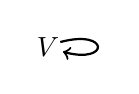
\begin{tikzpicture}[->,thick,xscale=1.3,
      yscale=1.3] \node (1)
  {$V$\!\!}; \path (1)
    edge [loop right]
(1);
\end{tikzpicture}}\!\!
{\cal B}_t$) if the number of dashed
  arrows in $\cal A$ is
  \textcolor{blue}{even};

  \item \alert{consimilarity transformations}
      (i.e., $\!\!\raisebox{-1.7mm}
{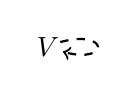
\begin{tikzpicture}[->,thick,xscale=1.3,
      yscale=1.3] \node (1)
  {$V$\!\!}; \path
    (1) edge [dashed,loop right]
(1);
\end{tikzpicture}}\!\!{\cal B}_t$)
if the number of dashed arrows in
  $\cal A$ is
  \textcolor{blue}{odd}.
\end{itemize}
\vspace{0.5cm}

A canonical form  for similarity
is given by Jordan's theorem.
\end{frame}


\begin{frame}

\frametitle{A canonical form  for consimilarity
is given in}


\begin{itemize}
  \item \alert{Y.P. Hong, R.A.
      Horn},{\it A canonical form
      for matrices under
      consimilarity}, Linear
      Algebra Appl. 102 (1988)
      143--168.
  \item \alert{R.A. Horn, C.R.
      Johnson},{\it Matrix
      Analysis, 2nd ed.}, Cambridge
      University Press, New York,
      2012.
\end{itemize}

\vspace{0.8cm}

 \textcolor{blue}{\it Each square
complex matrix is consimilar to a
direct sum, uniquely determined up to
permutation of direct summands, of
matrices of the following types:
\begin{itemize}
  \item $\alert{J_k(\lambda)}$, in
      which $\alert{\lambda\ge 0}$,
      and
  \item $\alert{
\begin{bmatrix} 0&1\\\mu
&0\end{bmatrix}}$,  in which
      $\alert{\mu\notin\mathbb R}$
      or $\alert{\mu<0}$.
\end{itemize}}

\end{frame}

\begin{frame}

\frametitle{Let $\cal
A$ be indecomposable into a direct
sum and\\ let there exist a singular ${\cal
A}_i$}


\textcolor{blue}{Lemma \\{\it There
are bases of $V_1,\dots,V_t$ in which
the matrix $A_i$ of each ${\cal A}_i$
possesses the property: all entries are
only 0's and 1's with at most one 1 in
each row and each column.}} \bigskip

\begin{corollary}
\begin{itemize}

  \item Each ${\cal A}_i$ maps a
      basis vector to a basis
      vector or $0$.
\item Each ${\cal A}_i$
    \alert{cannot map distinct}
    basis vectors to \alert{the
    same} basis vector:
$$
\xymatrix@R=6pt{
e_1\ar[rd]^{{\cal A}_i}&&\\
&f&\ \text{--- \alert{impossible}}\\
e_2\ar[ru]^{{\cal A}_i}&&\\}
$$
\end{itemize}
\end{corollary}
(i.e., the arrows must be parallel)
\end{frame}

\begin{frame}
\frametitle{Let there exist a singular ${\cal
A}_i$}

Construct the \alert{directed graph},
\begin{itemize}
  \item its
      \textcolor{blue}{vertices are
      basis vectors of
      $V_1,\dots,V_t$ from Lemma},
  \item there is an
      \textcolor{blue}{arrow from
      \alert{$u$} to \alert{$v$} if
      and only if $\exists{\cal
      A}_i:\alert{u}\mapsto\alert{v}$}.
\end{itemize}
\bigskip

By Lemma, the graph is a \alert{DISJOINT UNION OF CHAINS!!!}.

Since ${\cal{A}}$ is indecomposable,
the graph is connected, and so
\alert{it is a chain}.
\bigskip

Consider chains for the cycle
\[
\textcolor{blue}{\xymatrix@R=6pt@C=17pt{
&&V_1\ar@{<-}[rr]^{\alert{{\cal
      A}_2}}&&
V_2\ar@{<--}[dr]^{\alert{{\cal
      A}_3}}&\\
V_3\ar@{->}[urr]^{\alert{{\cal
      A}_1}}&&&&&
V_4\ar@{->}[dll]_{\alert{{\cal
      A}_4}}\\
& V_5\ar@{<--}[ul]_{\alert{{\cal
      A}_6}}&&
 V_6\ar@{<--}[ll]_{\alert{{\cal
      A}_5}}&&\\}}
\]


\end{frame}

\begin{frame}
\frametitle{Type I: A chain stops
exactly before the starting point; an
example}\vspace{-1cm}

\[\quad
\textcolor{blue}{\xymatrix@R=6pt@C=35pt{
&&e_{21}\ar@{<-}[rr]&&e_{31}
\ar@{<--}[ddr]&\\
e_{11}\ar@{->}[rru]&&e_{22}
\ar@{<-}[rr]&&e_{32}
\ar@{<--}[ddr]&\\
e_{12}\ar@{->}[urr]&e_{61}
\ar@{<--}[ul]
&&&&
e_{41}\ar@{->}[dll]\\
&e_{62}\ar@{<--}[ul]&&
e_{51}\ar@{<--}[ll]&&e_{42}
\ar@{->}[dll]\\
&&&e_{52}\\}}
\]
Then
\[
\textcolor{blue}{\xymatrix@R=6pt@C=7pt{
&&\langle e_{21}, e_{22}\rangle\ar@{<-}[rr]^{\alert{I_2}}&&
\langle e_{31}, e_{32}\rangle\ar@{<--}[dr]^{\alert{I_2}}&\\
\langle e_{11}, e_{12}\rangle\ar@{->}[urr]^{\alert{I_2}}&&&&&
\langle e_{41}, e_{42}\rangle\ar@{->}[dll]_{\alert{I_2}}\\
&\langle e_{61}, e_{62}\rangle\ar@{<--}[ul]_{\alert{I_2}}&&
\langle e_{51}, e_{52}\rangle\ar@{<--}[ll]_{
\alert{\begin{bmatrix}
               0 & 1 \\
               0 & 0 \\
             \end{bmatrix}
}}&&\\}}
\]
\end{frame}

\begin{frame}
\frametitle{Type I: A chain stops
exactly before the starting point; the
general case}\vspace{-1cm}


\[
\textcolor{blue}{\xymatrix@R=6pt@C=17pt{
&&\mathbb C^n\ar@{<-}[rr]^{\alert{I_n}}&&
\mathbb C^n\ar@{<--}[dr]^{\alert{I_n}}&\\
\mathbb C^n\ar@{->}[urr]^{\alert{I_n}}&&&&&
\mathbb C^n\ar@{->}[dll]_{\alert{I_n}}\\
&\mathbb C^n\ar@{<--}[ul]_{\alert{I_n}}&&
\mathbb C^n\ar@{<--}[ll]_{\alert{J_n(0)}}&&\\}}
\]
\bigskip
\bigskip
\bigskip



The singular Jordan can be over any
arrow.

\end{frame}


\begin{frame}



\frametitle{Type II: A chain does not
stop exactly before the starting point;
an example}


\text{The
chain}\quad$\textcolor{blue}{\xymatrix@R=6pt{
&&V_2\ar@{<-}[rr]^{\alert{\mathcal A_2}}&&
V_3\ar@{<--}[dr]^{\mathcal A_3}&\\
V_1\ar@{->}[urr]^{\mathcal A_1}&&&&&
V_4\ar@{->}[dll]_{\mathcal A_4}\\
&V_6\ar@{<--}[ul]_{\mathcal A_6}&&
V_5\ar@{<--}[ll]_{\alert{\mathcal A_5}}&&\\}} $

gives the cycle\vspace{-5mm}


\[
\textcolor{blue}{\xymatrix@R=6pt@C=17pt{
&&\langle e_{21} \rangle \ar@{<-}[rr]^{\alert{R_2=\begin{bmatrix}
   0&1
    \end{bmatrix}}}&&
\langle e_{31},e_{32} \rangle \ar@{<--}[dr]^{\begin{bmatrix}
   1&0\\0&1
    \end{bmatrix}}&\\
\langle e_{11} \rangle \ar@{->}[urr]^{{\begin{bmatrix}
   1
    \end{bmatrix}}}&&&&&
\langle e_{41}, e_{42} \rangle \ar@{->}[dll]_{\begin{bmatrix}
   1&0\\0&1
    \end{bmatrix}}\\
&\langle e_{61} \rangle \ar@{<--}[ul]_{{\begin{bmatrix}
   1
    \end{bmatrix}}}&&
\langle e_{51},e_{52} \rangle \ar@{<--}[ll]_{\alert{L^T_2=\begin{bmatrix}
   1\\0
    \end{bmatrix}}}&&\\}}
\]


\end{frame}



\begin{frame}
\frametitle{Type II: A chain does not
stop exactly before the starting point;
the general case}%\vspace{-1cm}


Two arrows are assigned by $M$ and $N$;
the others by $I$:
\[
\textcolor{blue}{\xymatrix@R=6pt@C=17pt{
&&V\ar@{<-}[rr]^{\alert{M}}&&
V\ar@{<--}[dr]^{I}&\\
V\ar@{->}[urr]^{I}&&&&&
W\ar@{->}[dll]_{I}\\
&W\ar@{<--}[ul]_{I}&&
W\ar@{<--}[ll]_{\alert{N}}&&\\}}
\]

$ (\alert{M},\alert{N})=\left\{
          \begin{array}{ll}
            (R_n,L_n)\text{ or }
(R_n^T,L_n^T), & \hbox{if }
\alert{\xymatrix{
 {V}
 \ar@<0.4ex>[r]^{M}
 &{W}
 \ar@<0.4ex>@{<-}[l]^{N}}}
\\
            (R_n,L_n^T)\text{ or }
(R_n,L_n^T), &
\hbox{if }
\alert{\xymatrix{
 {V}
 \ar@<0.4ex>[r]^{M}
 &{W}
 \ar@<0.4ex>[l]^{N}}}
          \end{array}
        \right.
$,

where \[R_n:=\left[\begin{smallmatrix}
0&1&&0\\&\ddots&\ddots&\\0&&0&1
\end{smallmatrix}\right],\quad
L_n:=\left[\begin{smallmatrix}
1&0&&0\\&\ddots&\ddots&\\0&&1&0
\end{smallmatrix}\right]
\]
\end{frame}








\begin{frame}

\frametitle{The classification of
cycles}

\begin{theorem}
Each cycle of linear and semilinear
mappings is isomorphic to a direct sum,
determined uniquely up to isomorphisms
of summands, of indecomposable cycles
of the following types:
\begin{itemize}
  \item %
 $\textcolor{blue}{ \xymatrix
@C=40pt{
     V
\ar@{-}@/_2.0pc/[rrr]^{
\mathcal B_t }
\ar@{-}[r]^{\mathbb 1}
         &
     V
\ar@{-}[r]^{\mathbb 1}
         &
{\ \dots\ }
         &V
\ar@{-}[l]_{\mathbb 1}
}}
$
\medskip

in which \alert{$ \mathcal B_t $ is
given by a Jordan block or an
indecomposable canonical block
under consimilarity} if the number
of dashed arrows is \alert{even or
odd, respectively}.\medskip

  \item Cycles that are given by
      chains.

\end{itemize}

\end{theorem}

\end{frame}

\begin{frame}

\frametitle{ \alert{Known cases:} the classification of}
\vspace{-0.5cm}

\begin{itemize}
  \item  $
          \begin{array}{ll}
\textcolor{blue}{\xymatrix{
 {V}
 \ar@<0.4ex>[r]
 &{W}
 \ar@<0.4ex>@{->}[l]}}
          \end{array}
$ was given in
\medskip
\begin{itemize}
  \item {\it \alert{N.M. Dobrovol'skaya, V.A. Ponomarev}, A pair of
counter-operators (in Russian), Uspehi Mat. Nauk 20\\
 (no. 6) (1965) 80--86;}
  \item {\it \alert{R.A. Horn, D.I. Merino}, Contragredient equivalence:\\
a canonical form and some applications, Linear Algebra \\
Appl. 214 (1995) 43--92.}
\end{itemize}
\medskip
   \item \textcolor{blue}{arbitrary cycles of linear mappings} is well known in the theory of representations of quivers.
   \medskip
  \item  $
          \begin{array}{ll}
\textcolor{blue}{\xymatrix{
 {V}
 \ar@<0.4ex>[r]
 &{W}
 \ar@<0.4ex>@{<--}[l]}}
          \end{array}
$ was given in
\medskip
\begin{itemize}
  \item
{\it\alert{D.$\check{Z}$. Djokovi$\acute{c}$}, Classification of pairs consisting of a\\
linear and a semilinear map, Linear Algebra Appl. 20\\
(1978) 147--165.}
\end{itemize}
\end{itemize}
\end{frame}

\begin{frame}

\frametitle{\alert{Future research}: regularizing algorithm for cycles of linear and semilinear mappings}
\vspace{-1cm}
Paul Van Dooren in the article
\medskip

\begin{itemize}
  \item \textcolor{blue}{The computation of Kroneckers canonical form of a singular pencil, Linear Algebra
Appl. 27 (1979) 103--140.}
\end{itemize}
\medskip

gave an algorithm that for each matrix pencil constructs its \alert{regularizing decomposition}
into a direct sum of
\begin{itemize}
  \item \textcolor{blue}{a nonsingular pencil};
  \item \textcolor{blue}{Kronecker's singular indecomposable canonical pencils}.
\end{itemize}
\medskip

The algorithm uses only unitary
transformations, which improves its computational stability.



\end{frame}

\begin{frame}

\frametitle{\alert{Future research}: regularizing algorithm for cycles of \\
linear and semilinear mappings}

Van Dooren's algorithm was extended by
Sergeichuk to cycles of linear mappings:

\[
\textcolor{blue}{
\xymatrix{
{V_1}
\ar@{-}@/_1.5pc/[rrrr]
\ar@{-}[r]&
V_2\ar@{-}[r]&
{\ \dots\ }&{V_{t-1}}
\ar@{-}[l]
\ar@{-}[r]&{V_t}}}
\]
\medskip

in which $V_1 \dots V_t$
are complex vector spaces and each line is
\begin{itemize}
  \item a full arrow
      \alert{$\longrightarrow$} or
      \alert{$\longleftarrow$}.
\end{itemize}

\alert{I
will give an analogous algorithm and construct a regularizing
decomposition for cycles of linear and semilinear mappings:}
\[
\textcolor{blue}{
\xymatrix{
{V_1}
\ar@{-}@/_1.5pc/[rrrr]
\ar@{-}[r]&
V_2\ar@{-}[r]&
{\ \dots\ }&{V_{t-1}}
\ar@{-}[l]
\ar@{-}[r]&{V_t}}}
\]

in which each line is
\begin{itemize}
  \item a full arrow
      \alert{$\longrightarrow$},
      \alert{$\longleftarrow$}, or
  \item a dashed arrow
      \alert{$\dashrightarrow$},
      \alert{$\dashleftarrow$}.
\end{itemize}

\end{frame}





\begin{frame}

\begin{center}

 \LARGE
Thank you\\

for your attention!

\end{center}
\end{frame}


\end{document}

\begin{frame}

\frametitle{The classification of
semilinear operators}

\end{frame}
